% Report schematic (not an experimental result).
% Illustrates, for a generic grid of specimens organised by campaign
% (rows) and treatment group (columns), which specimens are held out
% as the test partition under each of the three evaluation regimes.
% The layout is illustrative only and does not reproduce the exact
% campaign/treatment specimen counts given in the dataset chapter.
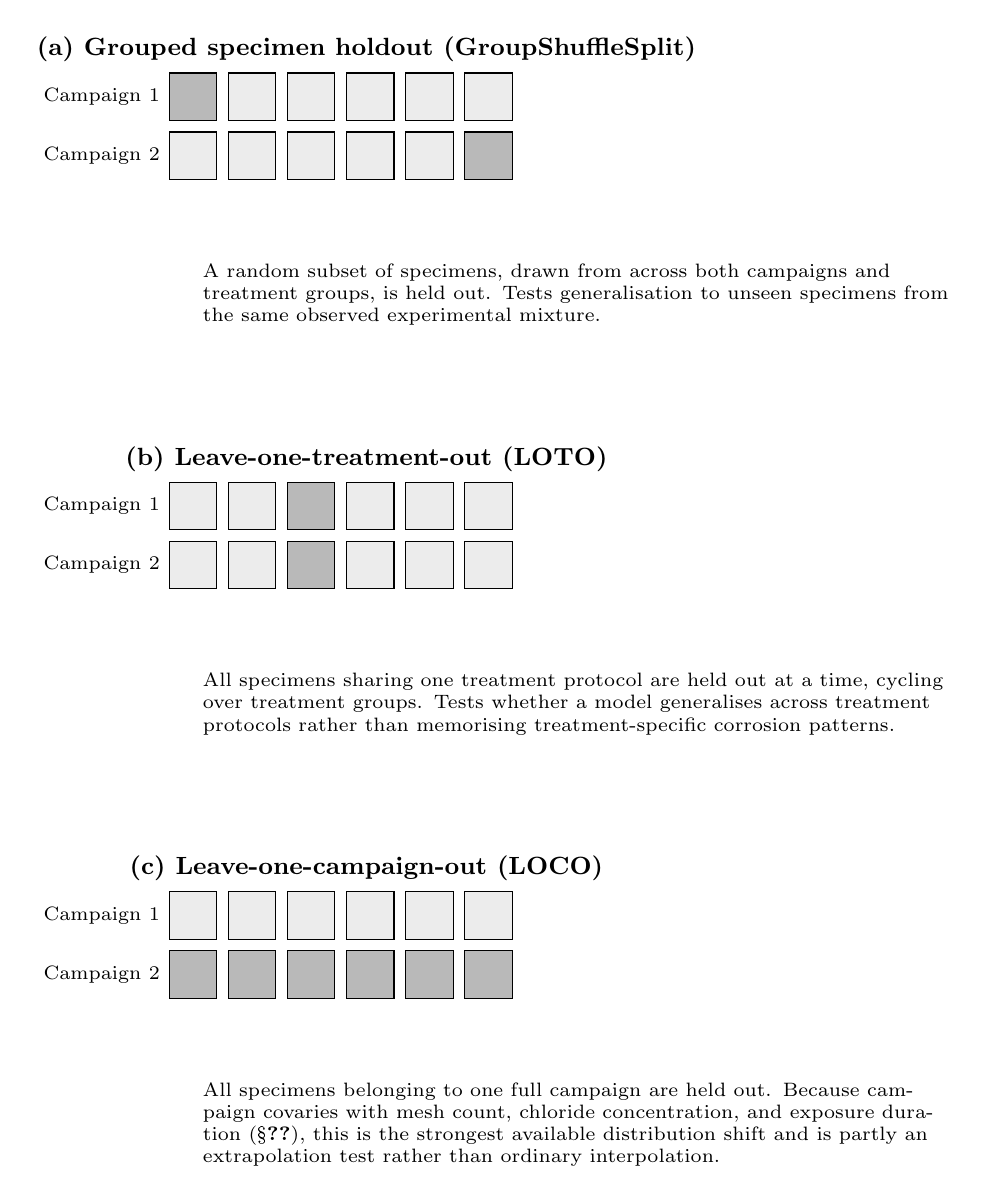
\begin{tikzpicture}[
    sq/.style={draw, minimum size=6mm, inner sep=0pt},
    train/.style={sq, fill=gray!15},
    held/.style={sq, fill=gray!55},
    panelcap/.style={font=\small\bfseries},
    rlbl/.style={font=\scriptsize, anchor=east},
    clbl/.style={font=\scriptsize, anchor=south}
]

\def\ncols{6}

% --- Panel (a): GroupShuffleSplit ---
\node[panelcap] at (2.2,0.6) {(a) Grouped specimen holdout (GroupShuffleSplit)};
\foreach \r/\rowname in {0/Campaign 1, 1/Campaign 2} {
    \node[rlbl] at (-0.3,-\r*0.75) {\rowname};
    \foreach \c in {0,...,5} {
        \pgfmathtruncatemacro{\isheld}{mod(\c+2*\r,7)==0}
        \ifnum\isheld=1
            \node[held] at (\c*0.75,-\r*0.75) {};
        \else
            \node[train] at (\c*0.75,-\r*0.75) {};
        \fi
    }
}
\node[font=\scriptsize, align=left, text width=9.5cm, anchor=north west]
    at (0,-2.0) {A random subset of specimens, drawn from across both
    campaigns and treatment groups, is held out. Tests generalisation
    to unseen specimens from the same observed experimental mixture.};

% --- Panel (b): LOTO ---
\begin{scope}[yshift=-5.2cm]
\node[panelcap] at (2.2,0.6) {(b) Leave-one-treatment-out (LOTO)};
\foreach \r/\rowname in {0/Campaign 1, 1/Campaign 2} {
    \node[rlbl] at (-0.3,-\r*0.75) {\rowname};
    \foreach \c in {0,...,5} {
        \ifnum\c=2
            \node[held] at (\c*0.75,-\r*0.75) {};
        \else
            \node[train] at (\c*0.75,-\r*0.75) {};
        \fi
    }
}
\node[font=\scriptsize, align=left, text width=9.5cm, anchor=north west]
    at (0,-2.0) {All specimens sharing one treatment protocol are held
    out at a time, cycling over treatment groups. Tests whether a model
    generalises across treatment protocols rather than memorising
    treatment-specific corrosion patterns.};
\end{scope}

% --- Panel (c): LOCO ---
\begin{scope}[yshift=-10.4cm]
\node[panelcap] at (2.2,0.6) {(c) Leave-one-campaign-out (LOCO)};
\foreach \r/\rowname in {0/Campaign 1, 1/Campaign 2} {
    \node[rlbl] at (-0.3,-\r*0.75) {\rowname};
    \foreach \c in {0,...,5} {
        \ifnum\r=1
            \node[held] at (\c*0.75,-\r*0.75) {};
        \else
            \node[train] at (\c*0.75,-\r*0.75) {};
        \fi
    }
}
\node[font=\scriptsize, align=left, text width=9.5cm, anchor=north west]
    at (0,-2.0) {All specimens belonging to one full campaign are held
    out. Because campaign covaries with mesh count, chloride
    concentration, and exposure duration (\S\ref{sec:confounding}), this
    is the strongest available distribution shift and is partly an
    extrapolation test rather than ordinary interpolation.};
\end{scope}

\end{tikzpicture}
